\documentclass[a4paper,oneside]{article}
\usepackage[utf8]{inputenc}
\usepackage[russian]{babel}
\usepackage{hyperref}
\usepackage{underscore}
\usepackage{setspace}
\usepackage{indentfirst} 
\usepackage{mathtools}
\usepackage{amsfonts}
\usepackage{enumitem}
% \usepackage[standard]{ntheorem}
\usepackage{amsthm}
\usepackage{cancel}
\usepackage{amssymb}
\usepackage[left=1.4cm,right=1.4cm,
    top=2.3cm,bottom=2.3cm,bindingoffset=0cm]{geometry}
\singlespacing

\usepackage{graphicx}
\graphicspath{ {./images/} }

\usepackage{fancyhdr}
\pagestyle{fancy}

\usepackage{tikz}
\usepackage{float}

\usepackage{tabularx}
\usepackage{tempora}
\newcommand{\bydef}{\stackrel{\text{по опр.}}{\implies}} % by definition - по определению
\newcommand{\parspace}{\vspace{10pt}}

\newcommand{\logor}{\vee}
\newcommand{\logand}{\wedge}

\newcommand{\imagin}{\mathrm{Im} \,}
\newcommand{\real}{\mathrm{Re} \,}

\newcommand{\dslim}{\displaystyle\lim}
\newcommand{\dslimn}{\dslim_{n \to \infty}}

\newcommand{\prop}[1]{#1^{\text{o}}}

\newcommand{\N}{\mathbb{N}}
\newcommand{\R}{\mathbb{R}}
\newcommand{\bb}[1]{\mathbb{#1}}

\newcommand{\eps}{\varepsilon}

\newcommand{\approach}[1]{\underset{#1}{\longrightarrow}}

% \theoremstyle{break}

% --- Теорема --- %
% \newtheoremstyle{break}% name
%   {}%         Space above, empty = `usual value'
%   {}%         Space below
%   {\itshape}% Body font
%   {}%         Indent amount (empty = no indent, \parindent = para indent)
%   {\bfseries}% Thm head font
%   {.}%        Punctuation after thm head
%   {\newline}% Space after thm head: \newline = linebreak
%   {}%         Thm head spec
% \theorembodyfont{\normalfont}
% \theoremstyle{break}
\newtheorem{theorem}{Теорема}[subsection]
% --------------- %

% --- Определение --- %
% \theorembodyfont{\normalfont}
\theoremstyle{definition}
\newtheorem{definition}{Определение}[subsection]
% ------------------- %

% --- Доказательство --- %
% \theoremheaderfont{\normalfont\itshape}
% \theorembodyfont{\normalfont}
% \newtheorem*{proof}{Доказательство.}
% ---------------------- %

% --- Пример --- %
\theoremstyle{definition}
\newtheorem*{example}{Пример}
% -------------- %

% --- Следствие --- %
% Corollary
% ----------------- %

% --- Замечание --- %
% Remark
\theoremstyle{definition}
\newtheorem*{remark}{Замечание}
% ----------------- %


\begin{document}

%----------------------------------------------------------------------------------------
%	TITLE PAGE
%----------------------------------------------------------------------------------------

\begin{titlepage} % Suppresses displaying the page number on the title page and the subsequent page counts as page 1
	\newcommand{\HRule}{\rule{\linewidth}{0.5mm}} % Defines a new command for horizontal lines, change thickness here
	
	\center % Centre everything on the page
	
	%------------------------------------------------
	%	Headings
	%------------------------------------------------
	
	\textsc{\LARGE Издательство Пупы и Лупы}\\[1.5cm] % Main heading such as the name of your university/college
	
	\textsc{\Large }\\[0.5cm] % Major heading such as course name
	
	\textsc{\large }\\[0.5cm] % Minor heading such as course title
	
	%------------------------------------------------
	%	Title
	%------------------------------------------------
	
	\HRule\\[0.4cm]
	
	{\huge\bfseries Лекции по дискретной математике}\\[0.4cm] % Title of your document
	
	\HRule\\[1.5cm]
	
	%------------------------------------------------
	%	Author(s)
	%------------------------------------------------
	
	\begin{minipage}{0.4\textwidth}
		\begin{flushleft}
			\large
			\textit{Автор}\\
			\textsc{Пупа} % Your name
		\end{flushleft}
	\end{minipage}
	~
	\begin{minipage}{0.4\textwidth}
		\begin{flushright}
			\large
			\textit{Редактор}\\
			\textsc{Лупа} % Supervisor's name
		\end{flushright}
	\end{minipage}
	
	% If you don't want a supervisor, uncomment the two lines below and comment the code above
	%{\large\textit{Author}}\\
	%John \textsc{Smith} % Your name
	
	%------------------------------------------------
	%	Date
	%------------------------------------------------
	
	\vfill\vfill\vfill % Position the date 3/4 down the remaining page
	
	{\large\today} % Date, change the \today to a set date if you want to be precise
	
	%------------------------------------------------
	%	Logo
	%------------------------------------------------
	
	%\vfill\vfill
	%\includegraphics[width=0.2\textwidth]{placeholder.jpg}\\[1cm] % Include a department/university logo - this will require the graphicx package
	 
	%----------------------------------------------------------------------------------------
	
	\vfill % Push the date up 1/4 of the remaining page
	
\end{titlepage}

%----------------------------------------------------------------------------------------

\section{Теория множеств}

\subsection{Множества и отношения между ними}

Множество "--- совокупность различаемых объектов.
Объекты называются его элементами.

Два множества равны ($A = B$), если:

\begin{equation*}
     \forall x: (x \in A \Leftrightarrow x \in B)
\end{equation*}

Множество $A$ включается в множество $B$ ($A \subseteq B$), если:

\begin{equation*}
    \forall x: (x\in A \Rightarrow x \in B)
\end{equation*}

Множество, $A$ строго включается в множество $B$ ($A \subset B$), если:

\begin{equation*}
    \forall x: (A \subseteq B ~ \& ~ A \neq B)
\end{equation*}

Множество называется пустым, если оно не содержит элементов.
Такое множество обозначается как $\varnothing$.

\begin{equation*}
    \forall A \neq \varnothing: ~ \varnothing \subseteq A
\end{equation*}

Некоторое множество $\Omega \neq \varnothing$ назовем универсальным множеством
и скажем, что

\begin{equation*}
    \forall A \neq \varnothing: ~ A \subseteq \Omega
\end{equation*}

\subsection{Операции над множествами}

Пусть $A, B \subseteq \Omega$:

\begin{equation*}
    A \cup B = \{ \forall~ x\in \Omega: ~ x \in A \logor x \in B \} \quad \text{(объединение)}
\end{equation*}

\begin{equation*}
    A\cap B = \{ \forall ~ x \in \Omega: ~ x \in A \logand x \in B \} \quad \text{(пересечение)}
\end{equation*}

\begin{equation*}
    \overline{A} = \{ \forall ~ x \in \Omega: ~ x \notin A \} \quad \text{(дополнение)}
\end{equation*}

\begin{equation*}
    A \setminus B = \{ \forall ~ x \in \Omega: ~ x\in A \logand x \notin B \} = 
    A \cup \overline{B}  \quad \text{(разность)} 
\end{equation*}

\begin{equation*}
    A \triangle B = \{ \forall ~ x \in \Omega: ~ x\in A \logand x\notin B \logor x \notin A 
    \logand x \in B \} \quad \text{(симметричная разность)}
\end{equation*}

Множество, содержащее конечное число элементов называется конечным.

Пусть $ A \neq \varnothing$ и $A$ состоит из $n$ элементов, тогда $|A| = n$ "---
мощность этого множества.

Множество при этом также обозначается как $A = \{ a_1, a_2, \dots, a_n\}$ или $A = \{x ~|~ P(x) \}$

Примеры:

\begin{equation*}
    A = \{ x \in \R ~|~ x\geq 0 \logand x \leq 1 \}
\end{equation*}

\subsection{Характеристические векторы множеств}

Пусть есть некоторое конечное множество $\Omega \neq \varnothing$ из $n$ элементов, 
$\Omega = \{ x_1, x_2, \dots, x_n\}$

Для удобства будем считать, что порядок перечисления множеств зафиксирован.

Теперь пусть $A \subseteq \Omega$.

Характеристическим вектором $A$ назовем булев вектор из $n$ компонентов 

\begin{equation*}
    \chi_A = (\chi_1^A, \chi_2^A, \dots, \chi_n^A), \text{~где } \chi_i^A = 
    \begin{cases}
        1, & x_i \in A \\
        0, & x_i \notin A 
    \end{cases}
\end{equation*}

Пусть $P(A)$ "--- множество всех подмножеств непустого множества $A$. 

Отметим, что $A \in P(\Omega)$

Пример:

$\Omega = \{a, b, c\}$

$P(\Omega) = 
\{ \varnothing, \{a\}, \{b\}, \{c\}, \{a, b\}, \{b, c\}, \{a, c\}, \{a, b, c\} \}$
\begin{center}
    \begin{tabularx}{0.2\textwidth}{c|c}
        $A$ & $\chi_A$ \\ \hline
        $\varnothing$ & $(0, 0, 0)$ \\
        $\{ a \}$ & $(1, 0, 0)$ \\  
        $\{ b \}$ & $(0, 1, 0)$ \\  
        $\{ c \}$ & $(0, 0, 1)$ \\  
        $\{ a,b \}$ & $(1, 1, 0)$ \\  
        $\{ b,c \}$ & $(0, 1, 1)$ \\  
        $\{ a,c \}$ & $(1, 0, 1)$ \\  
        $\{ a,b,c \}$ & $(1, 1, 1)$ \\  
    \end{tabularx}    
\end{center}

Стоит отметить, что данное отображение является биективным. 

\begin{theorem}[о числе подмножеств конечного множества]
    Число подмножеств $n$"=элементного множества равно $2^n$:

    \begin{equation*}
        |P(\Omega)| = 2^n
    \end{equation*}
    
\end{theorem}

Двоичной алгеброй называется $B_2 = \{ 0, 1\}$ с операциями $\{', +, \cdot\}$, где


\begin{itemize}
    \item <<$'$>> "--- логическое <<НЕ>>
    \item <<$+$>> "--- логическое <<ИЛИ>>
    \item <<$\cdot$>> "--- логическое <<И>>
\end{itemize}


Обозначим $B_2^n$ множество всех двоичных векторов длины $n$.

Пусть $\vec{a} = (a_1, a_2, \dots, a_n), \vec{b} = (b_1, b_2, \dots, b_n) 
\in B_2^n$

\begin{enumerate}
    \item $\vec{a}' = (a_1', a_2', \dots, a_n')$
    \item $\vec{a} + \vec{b} = (a_1 + b_1, a_2 + b_2, \dots, a_n + b_n )$
    \item $\vec{a} \cdot \vec{b} = (a_1 \cdot b_1, a_2 \cdot b_2, \dots, a_n \cdot b_n)$
\end{enumerate}

\begin{theorem}[О характеристических векторах]
    Пусть $\Omega \neq \varnothing$ (универсальное множество).
    Для любых непустых множеств $A, B \subseteq \Omega$ справедливо следующее:
    \begin{enumerate}
        \item $A = B \iff \chi_A = \chi_B$
        \item $\chi_{A\cup B} = \chi_A + \chi_B$
        \item $\chi_{A\cap B} = \chi_A \cdot \chi_B$
        \item $\chi_{\overline{A}} = (\chi_A)'$
        \item $\chi_\varnothing = (0, 0, \dots, 0) = \vec{0}$
        \item $\chi_\Omega = (1, 1, \dots, 1) = \vec{1}$
    \end{enumerate} 
\end{theorem}

Пример:

\begin{example}
Пусть $\Omega = \{ 1, 2, 3, 4, 5\}$, $A = \{1, 3, 4\}$, $B = \{ 1, 4, 5\}$.

Тогда $\chi_A = (1, 0, 1, 1, 0)$, $\chi_B = (1, 0, 0, 1, 1)$.

Получим:

$\chi_{\overline{A}} = (0, 1, 0, 0, 1)$

$\chi_{A \cup B} = (1, 0, 0, 1, 0)$

$\chi_{A \cap B} = (1, 0, 1, 1, 1)$
\end{example}

\subsection{Декартово произведение и отношения между множествами}

Пусть $A, B \neq \varnothing$. Декартовым произведением множеств $A$ и $B$
назовем множество упорядоченных пар 

\begin{equation*}
    A \times B = \{ ~(a, b) ~|~ a \in A \logand b \in B\}
\end{equation*}

$(a_1, b_1) = (a_2, b_2) \iff a_1 = a_2 \logand b_1 = b_2$

Очевидно, что если $|A| = n$, $|B| = m$, то $|A\times B| = n \times m$. 
Кроме того, $|P(A\times B)| = 2^{nm}$

Бинарным отношением между множествами $A$ и $B$ назовем любое подмножество
декартового произведения $\rho \subseteq |A \times B|$.

\subsection{Операции над бинарными отношениями}

Все теоретико"=множественные операции также справедливы для бинарных отношений.

\paragraph{Обращение бинарного отношения}

Пусть $\rho \subseteq A \times B$. Обратным отношением назовем 
$\rho^{-1} \subseteq B \times A~:~ \rho^{-1} = \{(b, a) \in B \times A ~|~ (a, b) \in \rho \}$

\begin{example}
    $A = \{1, 2, 3, 4\}$, $B = \{a, b , c\}$
    
    $\rho = \{(1, a), (1, b), (2, c), (4, b), (4, a)\}$
    
    $\rho = \{(a, 1), (b, 1), (c, 2), (b, 4), (a, 4)\}$


\end{example}

\paragraph{Операция умножения бинарных отношений}

Пусть $\rho \subseteq A \times B, \sigma \subseteq B \times C$. 
Определим операцию умножения бинарных отношений $\rho \cdot \sigma = 
\{(a, c) \in A \times C ~|~ \exists b ~:~ (a, b) \in \rho \logand (b, c) \in \sigma\}$

\subsection{Способы задания бинарных отношений}

\subsubsection{С помощью графов}

Пусть $\rho \subseteq A \times B$. $\vec{G}(\rho)$ "--- граф бинарного отношения.

Ребра такого графа "--- элементы множества $A$ и $B$, а ребра "--- ориентированные дуги 
из вершин из множества $A$ в вершины множества $B$.

\subsubsection{Двоичная булева матрица}

Двоичная матрица "--- матрица из $n$ строк и $m$ стобцов.

Определим следующую операцию: $(M)_{il}$ "--- элемент, находящийся на пересечении $i$ строки и $j$ столбца.

Пусть имеются матрицы $N$ и $M$. Определим следующие операции:

\begin{itemize}
    \item Дополнением матрицы называется $M'$, у которой $(M')_{ij} = (M)'_{i, j}$
    \item Суммой двух матриц называется $(M + N)_{A + B}$ такая, что $M_{ij} = N_{ij} + M_{ij}$
    \item Операциией пересечения матриц называется $(M \logand N)_{ij} = M_{ij} \cdot N_{ij}$.
    \item Транспонированием матриц называется $(M^T)_{ij} = M_{ji}$
    \item Пусть существуют матрицы $M_{n \times m}$ и $N_{m \times p}$. Определим произведение
    матриц как $\displaystyle M \cdot N = (M \cdot N)_{ij} = \sum_{k = 1}^m(M_{ik}) * N_{kj}$
\end{itemize}

Пусть множества $A$ и $B$ непустые и $\rho \subseteq A \times B$. 
Матрицей бинарного отношения назовем двоичную матрицу $M(\rho)$ и
определим её следующим образом 
\begin{equation}
    (M(\rho))_{ij} = \begin{cases}
        1, & (a_i, b_j) \in \rho \\
        0, & (a_i, b_j) \notin \rho
    \end{cases}
\end{equation}

Пусть $A$ "--- множество мощности $n$, $B$ "--- множество мощности m.
$A = \{a_1, \dots, a_n\}, B = \{b_1, \dots, b_m\}$.

$M(\rho)$ "--- матрица размерности $n \times m$

\begin{example}
    $A = \{1, 2, 3, 4\}$, $B = \{a, b, c\}$

    $\rho = \{(1, a), (1, b), (3, b), (4, a), (4, c)\}$
\end{example}


\begin{equation*}
    M(\rho) = \left( \begin{matrix}
        1 & 1 & 0 \\
        0 & 0 & 0 \\
        0 & 1 & 0 \\
        1 & 0 & 1 
    \end{matrix} \right)
\end{equation*}

\begin{theorem}{О матрицах бинарных отношений}
    Пусть $A$ и $B$ непустые множества и $\rho, \sigma \subseteq A \times B$,
    $\tau \subseteq B \times C$
    \begin{itemize}
        \item $\rho = \sigma \Leftrightarrow M(\rho) = M(\sigma)$
        \item Матрица дополнения бинарного отношения $M(\rho')
        = (M(\rho))'$
        \item $M(\rho \cap \sigma = M(\rho) \logand M(\sigma)$
        \item $(M\rho \cup \sigma = M(\rho) \logor M(\sigma))$
        \item $M(\rho^{-1}) = (M(\rho))^T$
        \item $M(\rho \cdot \tau) = M(\rho) \cdot M(\sigma)$
        \item $M(A \times B) = 1$
        \item $M(\varnothing) = 0$
    \end{itemize}

\end{theorem}

\begin{definition}
    Пусть $A$ и $B$ непустые множества $\rho \subseteq A \times B$.
    Первую(вторую) проекцию $\rho$ определим следующим образом:
    \begin{equation*}
        {pr_1}\rho =
         \{a(b) \in A(B) ~|~ \exists b(a) \in B(A) ~:~ (a, b) \in \rho\}
    \end{equation*}
\end{definition}

\begin{definition}
    $\rho$ называется 1(2)"=полным отношением, если $pr_1(2)\rho = A(B)$
\end{definition}

\begin{definition}
    Пусть $a \in A$. Срезом бинарного отношения $\rho \subseteq A \times B$ назовем
    множество, определяемое следующим образом:

    \begin{equation*}
        \rho(a) = \{b \in B ~|~ (a, b) \in \rho\}
    \end{equation*}
\end{definition}

\begin{definition}
    Бинарное отношение $\rho$ называется однозначным, если 
    $\forall a \in A ~| \rho(a)| \leq 1$
\end{definition}

Легко заметить, что если в матрице бинарного отношения не больше чем 1 единица,
то бинарное отношение является однозначным.

\begin{definition}
    Бинарное отношение $\rho$ называется обратнооднозначным, если обратное ему
    отношение является однозначным.
\end{definition}

Аналогичные рассуждения о матрицах можно привести и в этом случае.

\begin{definition}
    Бинарное отношение $\rho$ является взаимнооднозначным, если оно однозначно
    и обратнооднозначно.
\end{definition}

\begin{definition}
    Бинарное отношение называется отображением, если оно 1"=полно и однозначно.
\end{definition}

\begin{definition}
    Бинарное отношение $\rho$ называется инъективным (инъекцией), если $\rho$ является
    взаимнооднозначным отображением.
\end{definition}

$\rho$ называется сюръекцией, если оно 2"=полное + отображение.

Отображение, которое является одновременно инъекцией и 
сюръекцией (взаимооднозначным соответствием).

Из определения инъекцией $\forall a, b \in A (a \neq b) \rightarrow \rho(a) \neq \rho(b)$.

\paragraph{Отношение на множестве}

Пусть $A$ "--- непустое множество. Любое подмножество $A \times A$
называется отношением на множество $A$.

$|P(A \times A)| = 2^{n^2}$






















    

\section{Конечные автоматы}

\subsection{Конечные детерменированные автоматы}

Конечным детерменированным автоматом 
называется пятерка объектов $A = (S, X, Y, \delta, \lambda)$, где
$S$, $X$, $Y$ "--- конечные непустые множества, 

$S$ "--- множество состояния
автомата, а его элементы "--- состояния автомата.

$X$ "--- входной алфавит(множество входных сигналов).

$Y$ "--- выходной алфавит(множество выходных сигналов).

$\delta$ и $\lambda$ "--- функции переходов и выходов:

\begin{equation*}
    \delta: ~ S \times X \rightarrow S
\end{equation*}

\begin{equation*}
    \lambda: ~ S \times X \rightarrow Y
\end{equation*}

Автомат работает в дискретной временной шкале(в моменты времени $t_i \in \mathbb{N}$)
и в зависимости от того, в каком состоянии $S$ и какой сигнал $x \in X$ он получает, 
в следующий момент времени $t_{i+1}$ он перейдет в состояние $\delta(S, x)$ и
будет получено $\lambda(S, x)$ на выходе.

\subsection{Способы задания автоматов}

Автоматы можно задавать с помощью таблицы переходов-выходов или в виде
графа.

Рассмотрим эти способы.

\subsubsection{Таблица переходов автоматов}

Строки представляют из себя состояния автоматов, а столбцы "--- слова из множества $X$.

\begin{figure}[h!]
    \centering
    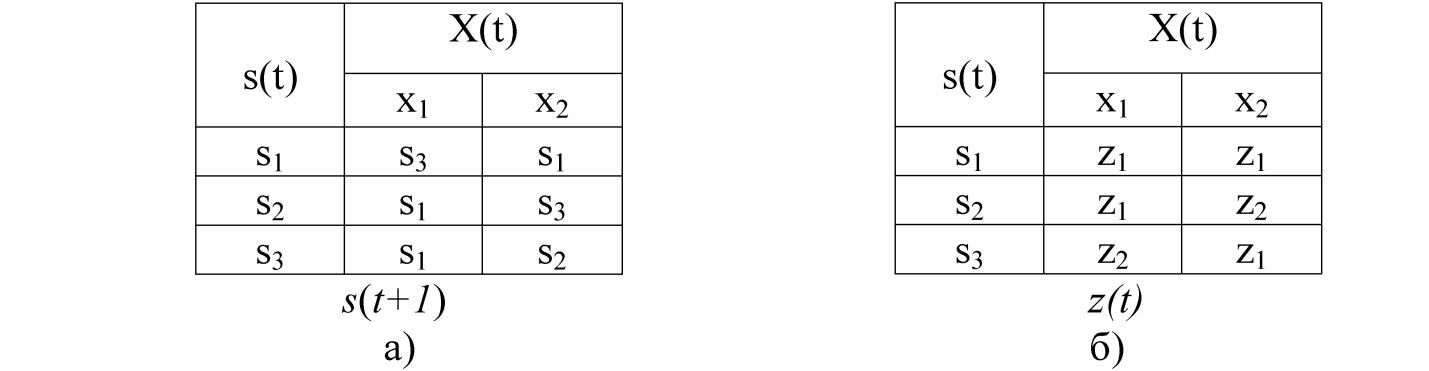
\includegraphics[scale=0.7]{table.png}
    \caption{Таблица переходов-выходов}
\end{figure}

\subsubsection{Граф автомата}

Вершинами являются элементы множества состояний, а ребра представляют из себя
пару элементов $(x,y) ~|~ x \in X, y \in Y$.


\begin{figure}[H]
    \centering
    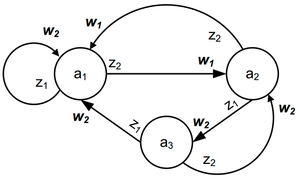
\includegraphics[scale=0.7]{graph.png}
    \caption{Граф автомата}
\end{figure}

Вершины "--- элементы множества состояний.

$\varepsilon$ "--- пустая цепочка (слово, которое не содержит ни одной буквы).

$|\varepsilon| = 0$


\begin{definition}
    Алфавитом назовем любое конечное непустое множество.
\end{definition}

\begin{definition}
    Словом над алфавитом $M$ назовем любую последовательность $p$ $x_1 x_2 \dots x_n$ такую, что
    $x_i \in M$. Если $p$ "--- слово над $M$, то длиной слова назовем количество
    букв этого слова и обозначим его как $|p|$.
\end{definition}

\begin{definition}
    Множество всех слов над алфавитом $M$ длины $k$ будем обозначать как $M^k$
\end{definition}

\begin{definition}
    Пусть $A(S, X, Y \delta, \lambda)$ "--- конечный детерменированный автомат.
    Продолженные (расширенные) функции переходов и выходов на слова входного
    алфавита $X$ определим индуктивно:
    
    $\delta(s, \varepsilon) = s$, $\delta(s, px) = \delta(\delta(s, p), x)
    ~\forall s \in S , ~p \in X^* ,~ x \in X$
\end{definition}

% Добавить примеры

\begin{definition}
    Два автомата $A_1$ и $A_2$ называются сравнимыми, если у них одинаковый
    входной и выходной алфавиты.
\end{definition}

\begin{definition}
    Будем говорить, что $A_1(S_1, X_1, Y_1, \delta_1, \lambda_1$ изоморфен
    автомату $A_2(S_2, X_2, Y_2, \delta_2, \lambda_2)$, если существует
    тройка биекций:
    \begin{equation*}
        \phi : ~ S_1 \rightarrow S_2
    \end{equation*}
    \begin{equation*}
        \psi : ~ X_1 \rightarrow X_2
    \end{equation*}
    \begin{equation*}
        \xi : ~ Y_1 \rightarrow Y_2
    \end{equation*}
    удовлетворяющая следующему условию:
    \begin{equation*}
        \forall s \in S_1, x \in X_1 : ~ \phi(\delta_1(s, x)) = \delta_2(\phi(s), \psi(x))
    \end{equation*}
    \begin{equation*}
        \forall s \in S_1, x \in X_1 : ~ \xi(\lambda_1(s, x)) = \lambda_2(\phi(s), \psi(x))
    \end{equation*}
\end{definition}

% Добавить рисунок


\begin{definition}
    Пусть $A_1$, $A_2$ "--- сравнимые автоматы. $A_1 \simeq A_2$, если
    $\exists \psi: ~ S_1 \rightarrow S_2$, что выполняется

    \begin{equation*}
        \forall s \in S, x \in X:~ \begin{matrix}
             \phi(\delta_1, (s, x)) = \delta_2(\phi(s), x) \\
             \lambda_1(s, x) = \lambda_2(\phi(s), x)
        \end{matrix}
    \end{equation*}
\end{definition}

\begin{theorem}[Об изоморфизме автоматов]
    Отношение изоморфизма на множестве всех автоматов есть отношение эквивалетности.
\end{theorem}

\begin{proof}
    Докажем, что для этого отношения характерны свойства отношения эквивалентности
    \begin{enumerate}
        \item Рефлексивность.
        
        $\begin{matrix}
            \phi : S_1 \rightarrow S_2 \\
            \psi : X_1 \rightarrow X_2 \\
            \xi : Y_1 \rightarrow Y_2 \\
        \end{matrix}$

        Покажем, что $\forall s \in S, x \in X$ выполняется

        \begin{equation*}
            \begin{matrix}
                \phi(\delta_1(s, x)) = \delta_2(\phi(s), \psi(x)) \\
                \xi(\lambda_1(s, x)) = \lambda_2(\phi(s), \psi(x))
            \end{matrix}
        \end{equation*}
            $\forall x \in X, y \in Y, s \in S: ~~~
            \begin{matrix}
                \phi(s) = s \\
                \psi(x) = x \\
                \xi(y) = y  
            \end{matrix} $

        Тогда 
        \begin{equation*}
            \begin{matrix}
                \phi(\delta(s, x)) = \delta(s, x) = \delta(\phi(x), \psi(s)) \\
                \xi(\lambda(s, x)) = \lambda(s, x) = \lambda(\phi(x), \xi(s))
            \end{matrix}
        \end{equation*}
        \item Симметричность.
        % TODO
    \end{enumerate}
\end{proof}


\paragraph{Утверждение}






\input{Equivalent.tex}
\input{Experiments.tex}

\end{document}